% -*- root: main.tex -*-

% \usepackage{showframe}

%%% Created by texsupport 20/09/2017

\makeatletter
\ifAJW@confsty
%
  \def\appendix{%
    \apptmp=\c@chapter %save chapter number
    \par
    \AJW@appendixtrue
    \def\section{\@startsection {section}{1}{\z@}
      {-30\p@ \@plus-7\p@ \@minus-3.5\p@}{8\p@}{\Aheadsize\bfseries\centering Appendix~}}
    \setcounter{section}{0}
    \@addtoreset{figure}{subsection}
    \setcounter{figure}{0}
    \setcounter{table}{0}
% set tocdepth to chapter heads only whether multi-author or single-author
    %\addtocontents{toc}{\protect\setcounter{tocdepth}{1}}
    \def\@chapapp{\appendixname}
    \def\thechapter {\Alph{chapter}}
    \def\thesection {\Alph{section}}
    \def\thesubsection {\Alph{section}.\arabic{subsection}}
    \def\thetable   {\Alph{section}.\@arabic\c@table}
    \def\thefigure  {\Alph{section}.\@arabic\c@figure}
    \def\theequation{\Alph{section}.\arabic{equation}}
}

% and only one appendix
  \def\oneappendix{\AJW@oneappendixtrue\appendix
    \def\thesection {}% remove the 'A' from Appendix heading
  }
\else
%
% single version
\def\appendix{\par\clearpage
 \AJW@appendixtrue
 \setcounter{chapter}{0}
 \setcounter{section}{0}
% set tocdepth to chapter heads only whether multi-author or single-author
 %\addtocontents{toc}{\protect\setcounter{tocdepth}{0}}
 \def\@chapapp{\appendixname}
 \def\thechapter {\Alph{chapter}}
 \def\thesection {\thechapter.\arabic{section}}
 \def\thetable   {\thechapter.\@arabic\c@table}
 \def\thefigure  {\thechapter.\@arabic\c@figure}
 \def\theequation{\thechapter.\arabic{equation}}
}
%
% and only one appendix
    \def\oneappendix{\AJW@oneappendixtrue\appendix}
\fi
\def\AJW@numberline#1{{\@hangfrom{\itshape \appendixname\ #1\ \quad}}}%% texsupport
\makeatother

\usepackage[pdftex,
            bookmarksnumbered=true,%% texsupport
            pdfauthor={Eric Peterson},
            pdftitle={Formal Geometry and Bordism Operations},
            pagebackref=true]{hyperref}

\usepackage[protrusion=true,expansion=true]{microtype}
% \usepackage{savetrees}
\usepackage{amsmath}
\usepackage{amssymb}
\usepackage{amsthm}
\usepackage{stmaryrd} % for \llbracket and \rrbracket
\usepackage{spectralsequences}

% \usepackage{mathpazo} % math & rm
% \linespread{1.05}        % Palatino needs more leading (space between lines)
% \usepackage[scaled]{helvet} % ss
% \usepackage{courier} % tt
% \normalfont
% \usepackage[T1]{fontenc}

\usepackage{newtxtext,newtxmath}

% \usepackage{mathptmx}

\usepackage{tikz}
\usetikzlibrary{matrix,calc,3d,arrows,positioning,fadings,shapes}

\usepackage{tikz-cd}
\makeatletter
\tikzcdset{
    iso/.style="\cong"{#1},
    iso'/.style="\cong"{/utils/exec=\isop@which,#1},
    equiv/.style="\simeq"{#1},
    equiv'/.style="\simeq"{/utils/exec=\isop@which,#1},
    % XXX: equal really breaks if you pair it with leftarrow.
    equal/.style={double distance=2pt,-}
}

\def\isop@getrow#1-#2-#3\@nil{#2}
\def\isop@getcolumn#1-#2-#3\@nil{#3}
\def\isop@which{
    \ifnum\@xp\isop@getrow\tikzcd@ar@start\@nil=\@xp\isop@getrow\tikzcd@ar@target\@nil\relax
        \pgfkeysalso{yscale=-1}
        \ifnum\@xp\isop@getcolumn\tikzcd@ar@start\@nil>\@xp\isop@getcolumn\tikzcd@ar@target\@nil\relax
            \pgfkeysalso{'}
        \fi
    \else
        \pgfkeysalso{'}
    \fi
}
\makeatother



\usepackage[disable]{todonotes}

\usepackage{pdflscape}
\usepackage[figuresright]{rotating}
\usepackage[mathic=true]{mathtools}

% used for \bigast
\usepackage{relsize}

% make the bibliography appear in the table of contents
\usepackage[nottoc,numbib]{tocbibind}

\usepackage{cleveref}
\usepackage{etoolbox}

% used to set custom chapter titles
\usepackage{tocloft,calc}

% this steals from http://tex.stackexchange.com/questions/36006/how-can-i-use-a-symbol-provided-by-a-package-without-changing-the-entire-mathema to import the "action" arrow
\DeclareFontFamily{U} {MnSymbolA}{}

\DeclareFontShape{U}{MnSymbolA}{m}{n}{
  <-6> MnSymbolA5
  <6-7> MnSymbolA6
  <7-8> MnSymbolA7
  <8-9> MnSymbolA8
  <9-10> MnSymbolA9
  <10-12> MnSymbolA10
  <12-> MnSymbolA12}{}
\DeclareFontShape{U}{MnSymbolA}{b}{n}{
  <-6> MnSymbolA-Bold5
  <6-7> MnSymbolA-Bold6
  <7-8> MnSymbolA-Bold7
  <8-9> MnSymbolA-Bold8
  <9-10> MnSymbolA-Bold9
  <10-12> MnSymbolA-Bold10
  <12-> MnSymbolA-Bold12}{}
\DeclareSymbolFont{MnSyA} {U} {MnSymbolA}{m}{n}
% 184 and 255 are both good options
\DeclareMathSymbol{\actson}{\mathrel}{MnSyA}{255}


\usepackage{booktabs}


\usepackage{epigraph}
\setlength\epigraphrule{0pt}


\usepackage{makeidx}
\makeindex

% REMOVE ME EVENTUALLY
% \usepackage{showidx}
% /REMOVE ME EVENTUALLY



%%% DONE WITH PACKAGES

% \setlength{\marginparwidth}{1in-\marginparsep} % fullpage sets margins to 1in

\setcounter{tocdepth}{1} % don't print subsections in the table of contents
\setcounter{secnumdepth}{1} % don't even bother numbering subsections

% todonotes definitions
\usepackage{xpatch}
\xpretocmd{\todo}{ }{}{} % fixes the \todo command gobbling a space

\newcommand{\oweproof}[1]{\todo[color=red]{\textbf{You owe a proof of: } #1.}}
\newcommand{\citeme}[1]{\todo[color=green]{\textbf{Cite me: } #1.}}
\newcommand{\needproof}[1]{\todo[color=magenta]{\textbf{I need to already know: } #1.}}


% symbol definitions

\input{letter-symbols.tex}

\setchars{\mathbb}{NZQRCSFPWH} % (or \setchars{\mathbb{#1}}{NZQRC} **)
\setchars{\mathcal}{LHO}  % (or \setchars{\mathcal{#1}}{O} **)
\setchars{\widehat{\mathbb{#1}}}{AG}
\setchars{\mathfrak}{mhp}

\newcommand{\barG}{\overline{\mathbb G}}
\newcommand{\RP}{\R\mathrm P}
\newcommand{\CP}{\C\mathrm P}
\newcommand{\HP}{\mathbb H\mathrm P}
\newcommand{\FH}{\textbf{FH}}
\newcommand{\UFH}{\textbf{UFH}}
\newcommand{\UGH}{\textbf{UGH}}
\newcommand{\CH}{\textbf{CH}}
\renewcommand{\t}{\mathbf t}
\newcommand{\Gm}{\mathbb G_m}
\newcommand{\Ga}{\mathbb G_a}
\newcommand{\ThomDivisor}{\mathbb D}
\renewcommand{\AA}{A\!\!A} % the right join of the leg and bar on the left letter should meet the left join of the leg and bar of the right letter

\newcommand{\<}{\langle}
\renewcommand{\>}{\rangle}
\newcommand{\sm}{\wedge}
\newcommand{\Susp}{\Sigma}
\newcommand{\Loops}{\Omega}
\renewcommand{\emptyset}{\varnothing}
\renewcommand{\phi}{\varphi}
\renewcommand{\epsilon}{\varepsilon}
\newcommand{\eps}{\varepsilon}
\newcommand{\mmod}{/\!\!/}
\newcommand{\co}{\colon\thinspace}
\newcommand{\into}{\hookrightarrow}
\newcommand{\cotensor}{\mathbin\square}
\newcommand{\from}{\leftarrow}
\newcommand{\onto}{\twoheadrightarrow}
\newcommand{\mhyphen}{\text{-}}
\newcommand{\Lk}{\Lambda_k}
\newcommand{\Lj}{\Lambda_j}
\newcommand{\adjunct}[4]{{#1}\colon\thinspace{#2} 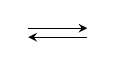
\begin{tikzpicture}[baseline] \draw[>=stealth,->] (0,1ex) -- (0.75,1ex); \draw[>=stealth,->] (0.75,0.25ex) -- (0,0.25ex); \end{tikzpicture}\ {#3}\thinspace\colon{#4}}

\renewcommand{\th}{\textsuperscript{th}}
% \newcommand{\st}{\textsuperscript{st}}
\newcommand{\nd}{\textsuperscript{nd}}
\def\Cech{\v{C}ech}

% from http://tex.stackexchange.com/questions/41186/big-asterisk-bigast-symbol
% these are magic numbers that depend upon the other geometry options
\newcommand{\bigast}{\mathop{\scalebox{2.5}{\raisebox{-0.35ex}{$\ast$}}}}

% cf http://tex.stackexchange.com/questions/286050/rotated-math-with-correct-font-size for sizing instructions
\newcommand{\circulatearrows}{\text{$\curvearrowleft$\hspace{-0.90em}\rotatebox[origin=bl]{180}{$\curvearrowleft$}}}

\newcommand{\context}[1]{\mathcal{M}_{#1}}
\newcommand{\Ucontext}[1]{\mathcal{UM}_{#1}}
\newcommand{\Econtext}[1]{E_\infty\mathcal{M}_{#1}}
\newcommand{\CatOf}[1]{\normalfont\textsc{#1}}
\newcommand{\ps}[1]{\llbracket{#1}\rrbracket}
\newcommand{\moduli}[1]{\mathcal{M}_{\mathbf{#1}}}
\newcommand{\OS}[2]{\underline{\smash{#1}}_{#2}}
\newcommand{\InternalHom}[1]{\operatorname{\underline{\smash{\CatOf{#1}}}}}
\newcommand{\InternalAut}{\operatorname{\underline{\smash{\operatorname{Aut}}}}}
\newcommand{\InternalEnd}{\operatorname{\underline{\smash{\operatorname{End}}}}}
\newcommand{\sheaf}[1]{\mathcal{#1}}
\newcommand{\stack}[1]{\mathcal{#1}}
\newcommand{\ThomSheaf}[1]{\mathbb{L}(#1)}

\newcommand{\SO}{\mathit{SO}}
\newcommand{\SU}{\mathit{SU}}
\newcommand{\Spin}{\mathit{Spin}}
\newcommand{\String}{\mathit{String}}
\newcommand{\TMF}{\mathit{TMF}}
\newcommand{\Tmf}{\mathit{Tmf}}
\newcommand{\tmf}{\mathit{tmf}}
\renewcommand{\top}{\mathrm{top}}
\renewcommand{\ss}{\mathrm{ss}}
\newcommand{\ord}{\mathrm{ord}}
\newcommand{\alg}{\mathrm{alg}}
\renewcommand{\ns}{\mathrm{ns}}
\newcommand{\TAF}{\mathit{TAF}}
\newcommand{\BP}{\mathit{BP}}
\newcommand{\MU}{\mathit{MU}}
\newcommand{\Tate}{\mathrm{Tate}}
\newcommand{\gl}{\mathit{gl}}
\newcommand{\GL}{\mathit{GL}}
\newcommand{\perf}{\mathrm{perf}}
\newcommand{\gpd}{\mathrm{gpd}}
\newcommand{\ptyp}{\mathit{p}\text{-}\mathrm{typ}}
\newcommand{\id}{\mathrm{id}}
\newcommand{\FGps}{\mathrm{FGps}}
\newcommand{\fin}{\mathrm{fin}}
\newcommand{\Res}{\mathrm{Res}}
\newcommand{\Tr}{\mathrm{Tr}}
\newcommand{\Cart}{\mathrm{Cart}}
\newcommand{\tr}{\mathrm{tr}}
\newcommand{\spin}{\mathit{spin}}
\newcommand{\EinftyRings}{E_\infty\CatOf{RingSpectra}}
\newcommand{\dx}{\operatorname{d\mathit{x}}}

\DeclareMathOperator{\Fix}{Fix}
\DeclareMathOperator{\Flag}{Flag}
\DeclareMathOperator{\im}{im}
\DeclareMathOperator{\Ind}{Ind}
\DeclareMathOperator{\Spec}{Spec}
\DeclareMathOperator{\Spf}{Spf}
\DeclareMathOperator{\Sch}{Sch}
\DeclareMathOperator*{\colim}{colim}
\DeclareMathOperator{\End}{End}
\DeclareMathOperator{\Div}{Div}
\DeclareMathOperator{\SDiv}{SDiv}
\DeclareMathOperator{\Sq}{Sq}
\DeclareMathOperator{\Sym}{Sym}
\DeclareMathOperator{\Aut}{Aut}
\DeclareMathOperator{\Def}{Def}
\DeclareMathOperator{\Pic}{Pic}
\DeclareMathOperator{\Ext}{Ext}
\DeclareMathOperator{\hAut}{hAut}
\DeclareMathOperator{\Coord}{Coord}
\DeclareMathOperator{\Tor}{Tor}
\DeclareMathOperator{\Cotor}{Cotor}
\DeclareMathOperator{\coker}{coker}
\DeclareMathOperator{\Hom}{Hom}
\DeclareMathOperator{\Weil}{Weil}
\DeclareMathOperator{\Alt}{Alt}
\DeclareMathOperator{\Tot}{Tot}
\DeclareMathOperator{\height}{ht}
\DeclareMathOperator{\Sub}{Sub}
\DeclareMathOperator{\Level}{Level}
\DeclareMathOperator{\Mono}{Mono}
\DeclareMathOperator{\Isog}{Isog}
\DeclareMathOperator{\Td}{Td}
\DeclareMathOperator{\cofib}{cofib}
\DeclareMathOperator{\SpH}{SpH}
\DeclareMathOperator{\Lie}{Lie}
\DeclareMathOperator{\Frob}{Frob}
\let\div\undefined\DeclareMathOperator{\div}{div}

% theorem environments

% \numberwithin{equation}{section}

\theoremstyle{plain}
\newtheorem{dummy}{Dummy}[section]
\newtheorem{theorem}[dummy]{Theorem}
\newtheorem{proposition}[dummy]{Proposition}
\newtheorem{lemma}[dummy]{Lemma}
\newtheorem{corollary}[dummy]{Corollary}
\newtheorem{conjecture}[dummy]{Conjecture}
\theoremstyle{definition}
\newtheorem{definition}[dummy]{Definition}
\newtheorem{construction}[dummy]{Construction}
\newtheorem{warning}[dummy]{Important Warning}
\theoremstyle{remark}
\newtheorem{remark}[dummy]{Remark}
\newtheorem{example}[dummy]{Example}

% sseqpages definitions

\DeclareSseqGroup\tower {m} {
    \class(0,0)
    \foreach \n in {1,...,#1} {
        \class(0,\n)
        \structline(0,\n-1)(0,\n)
    }
}

% \sseqnewgroup\tower[1]{
%     \class(0,0)
%     \foreach \y in {2,...,#1} {
%         \class(0, \y-1)
%         \structline(0, \y-2, -1)(0, \y-1, -1)
%     }
% }

\DeclareSseqCommand \etaclass { O{} }{
    \class[#1](\lastx+1,\lasty+1)
    \structline
}

% \sseqnewcmd\etaclass{
%     \class[class labels=above left,\options](\x,\y)
%     \structline(\x-1,\y-1,-1)(\x,\y,-1)
% }

% section headers

\crefname{section}{lecture}{lectures} \Crefname{section}{Lecture}{Lectures}
\crefname{chapter}{case study}{case studies} \Crefname{chapter}{Case Study}{Case Studies}

% put commas between adjacent footnotes without disturbing hyperref

\let\oldFootnote\footnote
\newcommand\nextToken\relax

\renewcommand\footnote[1]{%
    \oldFootnote{#1}\futurelet\nextToken\isFootnote}

\newcommand\isFootnote{%
    \ifx\footnote\nextToken\textsuperscript{,}%
    \else\ifx\footnotemark\nextToken\textsuperscript{,}\fi%
    \fi}

% from hood chatham: an \HFp macro that deals with subsequent subscripts intelligently

\makeatletter
\protected\def\HFp{H\mathbb{F}_p\@ifnextchar_{{}}{}}
\protected\def\HFtwo{H\mathbb{F}_2\@ifnextchar_{{}}{}}
\makeatother

% from hood chatham: place relevant spectral sequences on verso-recto pairs

\usepackage{afterpage}
\def\afterrectopage#1{{\ifodd\thepage#1\else\afterpage{#1}\fi}}

% from hood chatham: an \intertext command that works in tikzcd

% \usepackage{geometry}
\makeatletter
\edef\Gm@rmargin{\the\dimexpr1in + \hoffset + \oddsidemargin}
\edef\Gm@lmargin{\the\dimexpr1in + \hoffset + \oddsidemargin}
\makeatother
\RequirePackage{tikz-cd}
\RequirePackage{etoolbox}

\usetikzlibrary{calc}
\edef\mytikzcdrestoreat{\catcode`@=\the\catcode`@\let\noexpand\mytikzcdrestoreat\noexpand\undefined}
\makeatletter
\newbox\mytikzcd@trialbox

\patchcmd\tikzcd@{#1]}{remember picture,#1]\let\intertext\mytikzcd@intertext}{}{\errorfailedtopatch}



\def\mytikzcd@addtosavedpaths#1{\xdef\tikzcd@savedpaths{\unexpanded\expandafter{\tikzcd@savedpaths}#1}}
\def\mytikzcd@intertext{
	\@ifnextchar[{\mytikzcd@intertext@}{\mytikzcd@intertext@[0pt]}
}

\def\mytikzcd@intertext@[#1]#2{
	\setbox\mytikzcd@trialbox=\vbox{\hsize\textwidth #2}
	\expandafter\\\expandafter[\the\dimexpr\ht\mytikzcd@trialbox+\dp\mytikzcd@trialbox+#1]
    \edef\mytikzcd@lmargin{\if@mparswitch\ifodd\thepage\space \Gm@lmargin\else \Gm@rmargin\fi\else \Gm@lmargin\fi}
    \@xp\mytikzcd@findcolumn\@xp{\tikzcd@savedpaths}{1}
	\mytikzcd@addtosavedpaths{\unexpanded{\path[overlay] let \p1=(current page.west), \p2 =} (\noexpand\tikzcdmatrixname-\the\numexpr\pgfmatrixcurrentrow-1\relax-\mytikzcd@column), \noexpand\p3 = (\noexpand\tikzcdmatrixname-\the\pgfmatrixcurrentrow-1) in
	node[anchor=west,xshift=\mytikzcd@lmargin-2pt] at \unexpanded{(\x1,0.5*\y2+0.5*\y3) {\parbox{\textwidth}{#2}};}
	}
}


\def\mytikzcd@findcolumn#1#2{
    \def\mytikzcd@targetrow{#2}
    \expandafter\mytikzcd@findcolumn@\detokenize{#1\def\tikzcd@currentcolumn{x}\def\tikzcd@currentrow{6}}\@nil
}
\bgroup\lccode`\(=`\{\lccode`\)=`\}\lowercase{\egroup
\edef\mytikzcd@findcolumn@argspec{\unexpanded{#1}\detokenize{\def\tikzcd@currentcolumn}\unexpanded{(#2)}\detokenize{\def\tikzcd@currentrow}\unexpanded{(#3)}}
}

\@xp\def\@xp\mytikzcd@findcolumn@\mytikzcd@findcolumn@argspec{
    \expandafter\ifx\detokenize{x}#2
        \ifnum\mytikzcd@row<\the\numexpr\pgfmatrixcurrentrow-1\relax\def\mytikzcd@column{1}\fi
        \@xp\@gobbletonil
    \else
        \def\mytikzcd@column{#2}
        \def\mytikzcd@row{#3}
        \@xp\mytikzcd@findcolumn@
    \fi
}



\def\@gobbletonil#1\@nil{}
\mytikzcdrestoreat 

% from hood chatham: 

% taken from https://tex.stackexchange.com/a/164490/2671

\makeatletter
\newcommand{\sumfgl}[1]{\mathop{\vphantom{\sum}\mathpalette\sum@fgl{#1}}}
\newcommand{\sum@fgl}[2]{%
  \ooalign{%
    \sum@fgl@vc{#1}{\sum}\cr
    \hidewidth\sum@fgl@vc{\sum@fgl@next{#1}}{\mkern17mu#2}\hidewidth\cr}%
}
\newcommand{\sum@fgl@vc}[2]{%
  $\vcenter{\hbox{$\m@th#1#2$}}$%
}
\newcommand{\sum@fgl@next}[1]{%
  \ifx#1\displaystyle\scriptstyle\fi
  \ifx#1\textstyle\scriptscriptstyle\fi
  \ifx#1\scriptstyle\scriptscriptstyle\fi
  \ifx#1\scriptscriptstyle\scriptscriptstyle\fi
}
\def\sumphi{\sumfgl{\phi}}
\def\sumG{\sumfgl{\G}}
\def\sumGamma{\sumfgl{\Gamma}}
\makeatother




% from https://tex.stackexchange.com/questions/52076/how-to-make-a-superscript-on-the-upper-left-hand-corner-of-a-letter :

\def\presuper#1#2%
  {\mathop{}%
   \mathopen{\vphantom{#2}}^{#1}%
   \kern-\scriptspace%
   #2}

% from hood chatham: 
\makeatletter
\def\idxentry{\@ifnextchar[{\idxentry@}{\idxentry@dbl}}
% \def\idxentry@dbl#1{\mycommand@[#1]{#1}}
\def\idxentry@dbl#1{\textit{#1}\index{#1}}
\def\idxentry@[#1]#2{\textit{#2}\index{#1@#2}}
\makeatother

% from hood chatham: fix cleveref to work with cambridge7a
\makeatletter
\AtBeginDocument{%
\def\@thm{\@ifnextchar[{\cref@thmoptarg}{\cref@thmnoarg}}%]
\patchcmd\cref@thmoptarg {.}{\enskip}{}{\error}}
\makeatother

\makeatletter
\AtBeginDocument{%
\patchcmd{\@makechapterhead}{\huge\bfseries \thechapter}{\huge\bfseries \chaptername\ \thechapter}{}{\error}%
}
\makeatother

% set the default arrow style
\tikzset{>=stealth}
\tikzcdset{arrow style=tikz}

% put rectos back into \chapter
\makeatletter
\patchcmd{\chapter}{\clearpage}{\cleardoublepage}{}{\error}
\makeatother

% make footnotes fully justified
\makeatletter
\patchcmd{\cref@old@makefntext}{\raggedright}{\relax}{}{\error}
\makeatother

% make backrefs look pretty
\renewcommand*{\backref}[1]{}
\renewcommand*{\backrefalt}[4]{[%
    \ifcase #1 Not cited.%
          \or Cited on page~#2.%
          \else Cited on pages #2.%
    \fi%
    ]}

% allow large align* blocks to be broken across pages...
% ... but only from verso to recto!: https://tex.stackexchange.com/questions/224020/allow-displaybreak-only-from-even-to-odd-pages
\makeatletter
\everymath{%
  \ifodd\value{page}\allowdisplaybreaks[0]%
    \else \allowdisplaybreaks[4]%
  \fi
}
\makeatother


\usepackage{mdframed}
\newmdenv[
  topline=false,
  bottomline=false,
  skipabove=\topsep,
  skipbelow=\topsep
]{siderules}


